\newif\ifvimbug
\vimbugfalse

\ifvimbug
\begin{document}
\fi

\exercise{Expectation-Maximization}

In this exercise your task is to control a 2-DoF planar robot to throw a ball at a specific target. You will use an episodic setup, where you first specify the parameters of the policy, evaluate them on the simulated system, and obtain a reward. The robot will be controlled with the Dynamic Motor Primitives (DMPs).
The goal state of the DMPs is pre-specified and the weights of the DMP
$\theta_i, i = 1 \ldots 10$ are the open parameters of the control policy. Each DoF of the robot is controlled with a DMP with five basis functions. The ball is mounted at the end-effector of the robot and gets automatically released at time step $t_{\textrm{rel}}$.
We define a stochastic distribution $\pi(\vec{\theta}|\vec{\omega}) =
\mathcal{N}(\vec{\theta}|\vec{\mu},\boldsymbol{\Sigma})$, with $\omega = \{\vec{\mu},\boldsymbol{\Sigma} \}$. \\
Your task it to update the parameters $\vec{\omega}$ of the policy using EM to maximize the expected return. In this exercises we will not
modify the low-level control policy (the DMPs) of the robot. 

A template for the simulation of the 2-DoF planar robot and plotting functions can be found at the course website. For the programming exercises, attach snippets of your code.

\begin{questions}


\begin{question}{Analytical Derivation}{5}

Using the weighted ML estimate,
\begin{equation}
    \vec{\omega}_{k+1} = \underset{\vec \omega}{\arg\max} \{ \sum_i w^{[i]} \log \pi(\vec{\theta}^{[i]};\vec{\omega})\},
\end{equation}
derive analytically the update rule for our policy $\pi(\vec{\theta}|\vec{\omega})$ for the mean $\vec{\mu}$. Show your derivations.

\begin{answer}\end{answer}

\end{question}

%----------------------------------------------


\begin{question}{Programming Exercise}{15}
Implement the EM algorithm using the provided framework. Your goal is to throw the ball at $\vec x = [2,1]m$ at time $t=100$. Use the weighted Maximum Likelihood (ML) solutions for updating the parameters of the policy. For the mean, use the equation derived at the previous exercise. For the covariance, the update rule is 
\begin{equation}
	\vec \Sigma_\mathrm{new} = \frac{\sum_i w^{[i]} (\vec{\theta}^{[i]}-\vec{\mu}_{\mathrm{new}})     (\vec{\theta}^{[i]}-\vec{\mu}_{\mathrm{new}})^T}{\sum_i w^{[i]}}.
\end{equation}
To calculate the weights $\vec{w}_i$ for each sample, transform the returned rewards by 
\begin{equation}
	\vec w^{[i]} = \exp ( ( \vec{R}^{[i]}(\vec{\theta}) - \max(\vec{R}) ) \beta )
\end{equation}
where the vector $\vec R\in \mathbb{R}^{N \times 1}$ is constructed from the rewards of the $N$ samples. The
parameter $\beta$ is set to
\begin{equation}
	\beta = \frac{\lambda}{ \max(\vec{R}) - \min(\vec{R}) },
\end{equation}
where $\lambda = 7$. Start with the initial policy 
\begin{equation}
	\pi(\vec{\theta}|\vec{\omega}) = \mathcal{N}(\vec{\theta}|\vec{0}, 10^6  \vec{I})
\end{equation}
and calculate the average reward at each iteration. Iterate until convergence or for a maximum number of 100 iterations.
We assume that convergence is achieved when the average return does not change much at every iteration, i.e., 
$$ | <\vec{R}_{i-1}> - <\vec{R}_\textrm{i}> | < 10^{-3}, $$
where $<\cdot>$ denotes the average operator.
At each iteration use 
$ N = 25 $ samples. In order to avoid getting stuck to a local optimum, we force the algorithm to explore a bit more by adding a regularization factor to the covariance of the policy,
\begin{equation}
    \vec{\Sigma}_\mathrm{new}^\mathrm{'} = \vec{\Sigma}_\mathrm{new} + \vec{I}.
\end{equation}
What is the average return of the final policy? 
Use \texttt{animate\_fig} from \texttt{Pend2dBallThrowDMP.py} to show how the final policy of the robot looks like (attach all five screenshots).

\begin{answer}

	The average return of the final policy is: -39.4430848515 .\\
	\\
	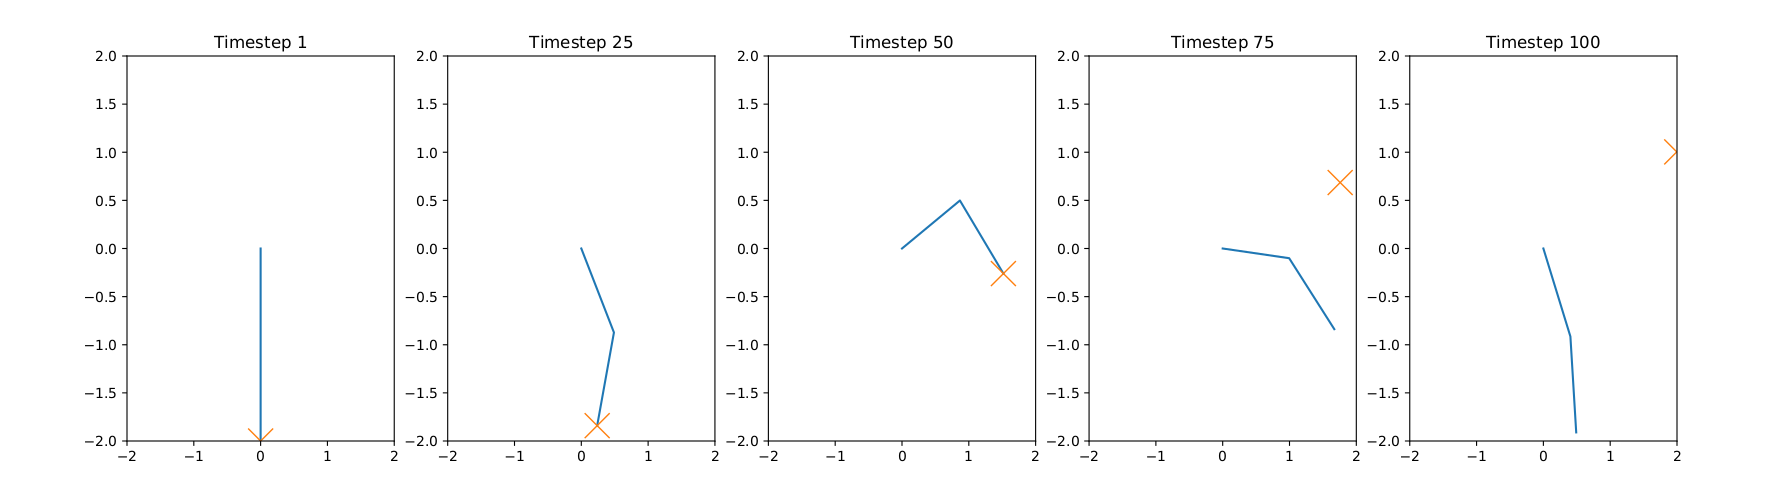
\includegraphics[width=174mm]{EM-l7.png}
	\lstinputlisting[language=Python,firstline=14,lastline=87]{../code/example_em.py}

\end{answer}

 \end{question}



%----------------------------------------------

\begin{question}{Programming Exercise}{5}
Repeat the learning 10 times and plot the mean of the average return of all runs with $95\%$ confidence.
Use the logarithmic scale for your plot.

    
\begin{answer}
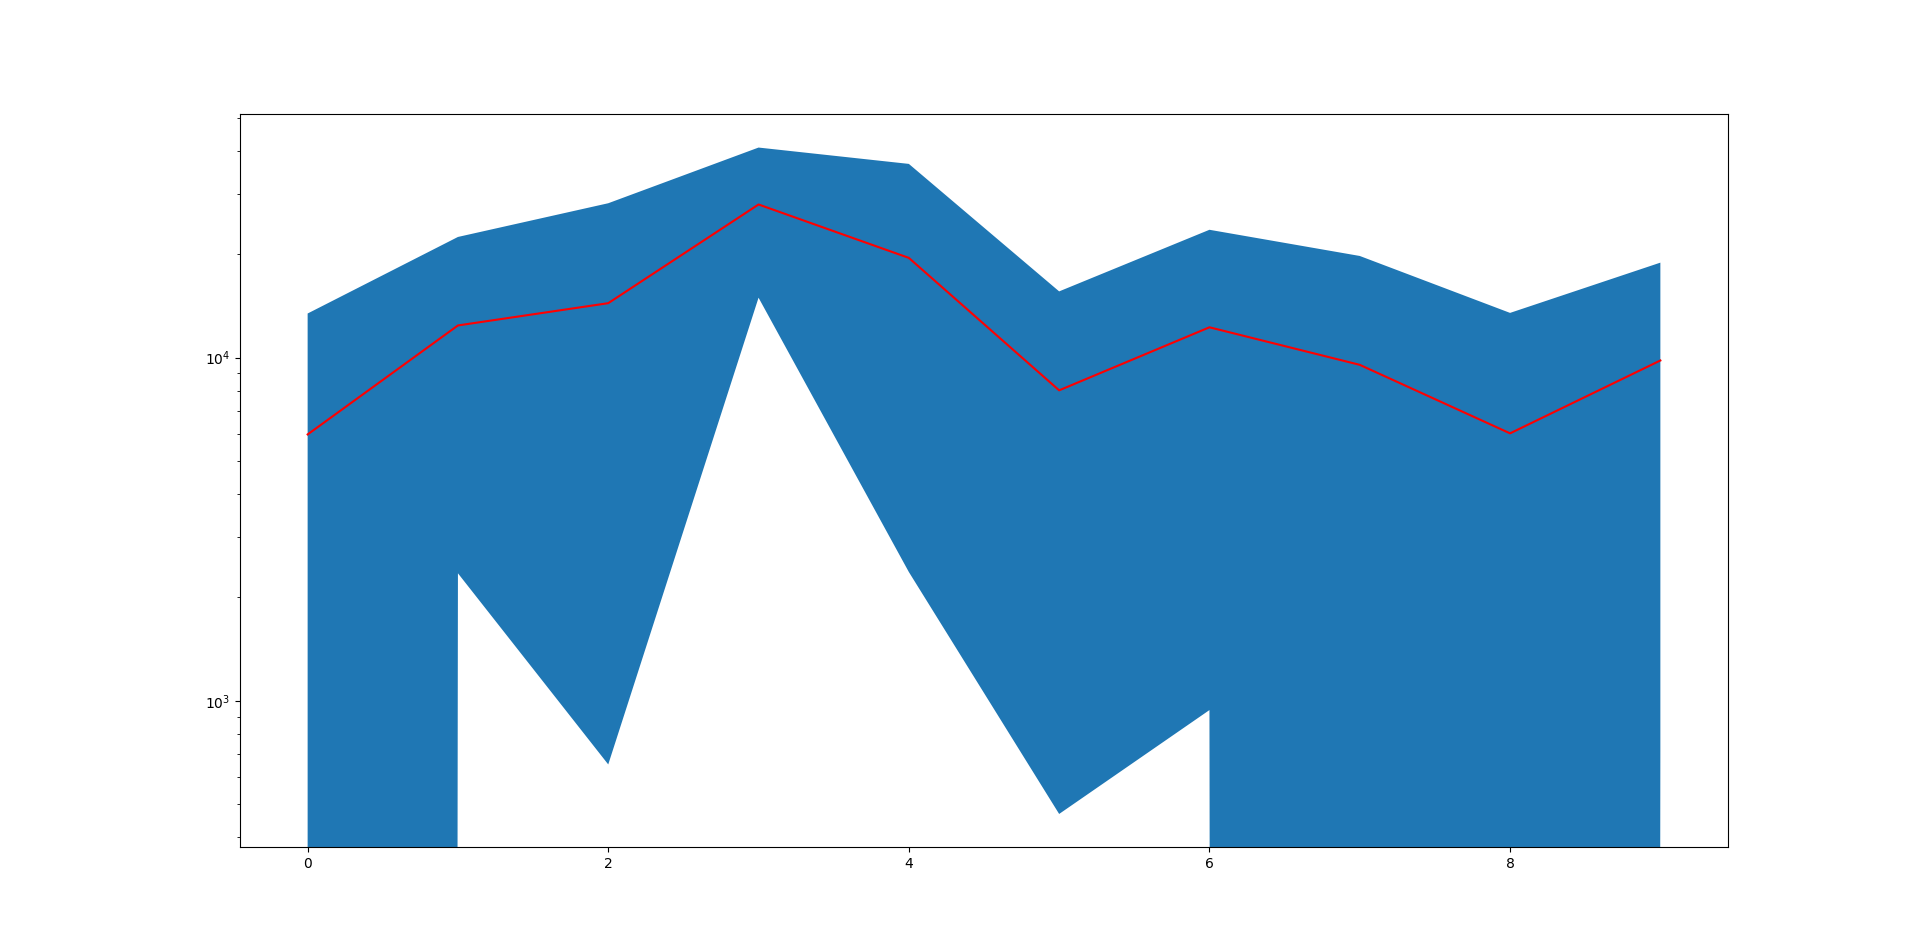
\includegraphics[width=174mm]{7-mean2.png}
Iterations on x-axis and negative reward on y-axis.\\
\lstinputlisting[language=Python,firstline=88,lastline=119]{../code/example_em.py}
\end{answer}

\end{question}



%----------------------------------------------

\begin{question}{Tuning The Temperature}{5}
Repeat the previous exercise with temperature $\lambda = 25$ and $\lambda = 3$. Plot in one figure the mean of the average returns for all $\lambda = 3$, $\lambda = 7$, $\lambda = 25$ with $95\%$ confidence.
How does the value of $\lambda$ affects the convergence of the algorithm in theory? 
Use the logarithmic scale for your plot.

\begin{answer}
The $\lambda$ coefficient (temperature) in theory affects the convergence kind of like a learning rate. So, if you choose a bigger temperature the algorithm converges faster. However, it could just stuck in a local optima, not a global one.	
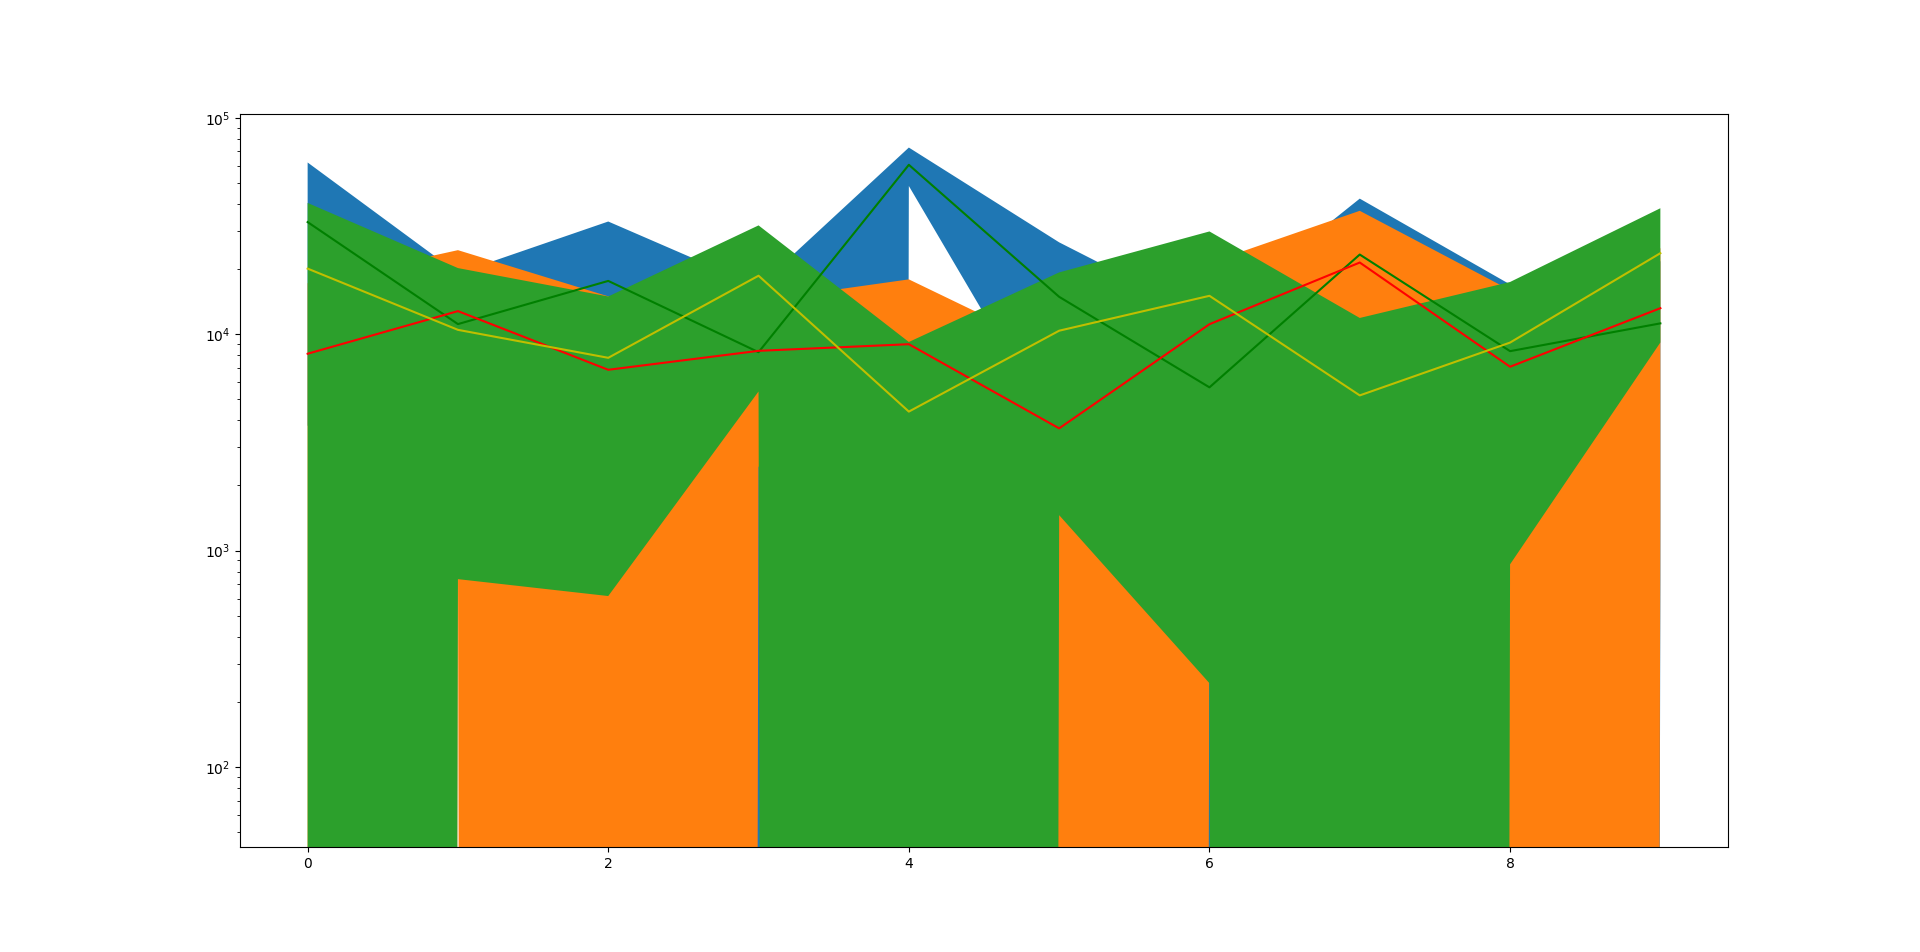
\includegraphics[width=174mm]{lambdas.png}
\end{answer}


\end{question}

%----------------------------------------------

\begin{question}[bonus]{Optimal Temperature}{5}
The problem of choosing $\lambda$ falls under a more general RL problem. Which one?
Which algorithm would allow you to automatically select the optimal $\lambda$? Explain it with your words.
Does it still have hyperparameters to be set?

\begin{answer}
It falls under the problem of hyperparameter tuning. 
\end{answer}


\end{question}


\end{questions}

